\documentclass[12pt]{article}
\usepackage[utf8]{inputenc}
\usepackage{amsmath}
\usepackage{amsfonts}
\usepackage[letterpaper, margin=2cm]{geometry}
\usepackage[shortlabels]{enumitem}

\setlength{\parindent}{0ex}
\setlength{\parskip}{1em}

\usepackage{Sweave}
\begin{document}
\Sconcordance{concordance:tavtigian.tex:tavtigian.Rnw:%
1 10 1 1 0 71 1 1 3 2 0 2 1 1 10 8 0 1 18 16 0 1 1 1 3 7 0 1 27 25 0 1 %
3 1 0 1 3 10 0 1 2 2 1 1 14 13 0 1 1 4 0 1 2 11 1 1 2 1 0 1 2 2 1 1 2 2 %
1 4 0 1 2 25 1 1 6 4 0 2 2 4 1 1 2 4 1 4 0 1 2 7 1 1 2 7 0 1 2 4 1 1 3 %
1 0 1 1 1 5 3 0 7 1 1 5 4 0 1 3 1 0 1 1 5 0 1 3 2 1 1 2 1 0 1 1 1 3 2 0 %
1 1 16 0 1 2 12 1}


\section*{Adapting Tavtigian et al.'s Bayesian System for LLRs}

\subsection*{Background}

We recently developed a method to translate variant effect scores from VE maps
into measures of log likelihood of pathogenicity based on the densities of
positive and negative reference variants across the VE map's score spectrum.
The goal behind these efforts was to provide a more useful metric for variant
classification. These classifications however are classically based on the ACMG
guidelines which only use simple categories.

Tavtigian et al. 2018 previously introduced the idea of representing the ACMG
variant classification guidelines as a Bayesian framework. They based this on
equating the different evidence levels (Pathogenic-Very Strong, Pathogenic-Strong,
Pathogenic-Moderate, Pathogenic-Supporting, Benign-Supporting, and Benign-Strong)
to different thresholds of what they call Odds of Pathogenicity or OddsPath (OP).

They state a number of modeling goals, which are based on the ACMG's loose
definition of the `Pathogenic' classification as corresponding to a greater than
99\% chance of being pathogenic, and `Likely pathogenic' as corresponding to a
greater than 90\% chance of being pathogenic. This means a successful model
should fulfill the following criteria:
\begin{enumerate}[(A)]
  \item Evidence combination rules with the same classification outcome
  (e.g. likely pathogenic) should ideally yield the same lower bound on
  posterior probability.
  \item Evidence combination rules for `Likely Pathogenic' should yield
  posteriors greater than $90\%$.
  \item Evidence combination rules for `Pathogenic' should yield posteriors
  greater than $99\%$.
\end{enumerate}

A quick examination of Tavtigian et al.'s underlying methods shows that what
they refer to as `OddsPath' (OP) is just another name for the likelihood ratio
$$\frac{P(Data|Pathogenic)}{P(Data|Benign)}$$, often also referred to as the
Bayes Factor, or $\Lambda$. This makes it easy for us to adopt to our existing
LLR metric, since the log Likelihood Ratio (LLR) is simply $\log(\Lambda)$.

The authors make a number of modeling decisions:
\begin{enumerate}
  \item Adjacent evidence levels should scale in OP exponentially by a power
  of $X$. That means our equivalent LLRs scale multiplicatively by $X$.
  \item ACMG rules for evidence combination work by multiplying OPs. That means
  our equivalent LLRs will be combined by addition.
\end{enumerate}

Next they have to pick a number of modeling parameters. The parameters to choose are:
\begin{enumerate}
  \item The scaling factor $X$.
  \item An underlying prior probability of pathogenicity $P_{prior}$.
  \item A starting point for their OP scale from which all other OP thresholds
  follow. For this they pick highest pathogenic evidence level Pathogenic-Very
  strong $OP_{PVSt}$.
\end{enumerate}

For the scaling factor, they choose $X=2$. This is because it does best at fulfilling criterion (A).

For the prior, they more or less arbitrarily pick $P_{prior}=0.1$. The authors
claim that they roughly base this on the prevalence of pathogenic variants in BRCA1
and BRCA2.

Finally, they have to choose a starting point for their OP scale, which they do by picking an arbitrary OP for the Pathogenic-Very strong ($OP_{PVSt}=350$). This number was picked because it fulfilled criteria (B) and (C) given their choice of X and
the prior.

\subsection*{Re-implementation with LLRs}

We can quickly test that by choosing the same parameters, our LLR-based
implementation yields the exact same results for the combination rules:

\begin{Schunk}
\begin{Sinput}
> #Modeling parameters
> prior <- 0.1
> LLRpvst <- log10(350)
> X <- 2
> #function to calculate posterior given prior and LLR
> llr2post <- function(llr,prior=0.1) {
+   #log prior odds
+ 	lpo <- log10(prior/(1-prior))
+ 	#posterior odds
+ 	posto <- 10^(llr+lpo)
+ 	#posterior prob
+ 	(posto) / (1+posto)
+ }
> #here we derive the LLR evidence thresholds based on our parameters
> calcThresholds <- function(LLRpvst,X) {
+   list(
+     #pathogenic very strong
+   	LLRpvst=LLRpvst,
+   	#pathogenic strong
+   	LLRpst=LLRpvst/X,
+   	#pathogenic moderate
+   	LLRpm=LLRpvst/(X^2),
+   	#pathogenic supporting
+   	LLRpsu=LLRpvst/(X^3),
+   	#benign supporting
+   	LLRbsu=-LLRpvst/(X^3),
+   	#benign strong
+   	LLRbst=-LLRpvst/(X^1)
+   )
+ }
> thresholds <- calcThresholds(LLRpvst,X)
> #print thresholds
> round(unlist(thresholds),digits=3)
\end{Sinput}
\begin{Soutput}
LLRpvst  LLRpst   LLRpm  LLRpsu  LLRbsu  LLRbst 
  2.544   1.272   0.636   0.318  -0.318  -1.272 
\end{Soutput}
\begin{Sinput}
> #test evidence combination rules
> calcComboLLRs <- function(thresholds) {
+   with(thresholds,c(
+     #pathogenic combinations
+   	path1a=LLRpvst+LLRpst,
+   	path1b=LLRpvst+2*LLRpm,
+   	path1c=LLRpvst+LLRpm+LLRpsu,
+   	path1d=LLRpvst+2*LLRpsu,
+   	path2 =2*LLRpst,
+   	path3a=LLRpst+3*LLRpm,
+   	path3b=LLRpst+2*LLRpm+2*LLRpsu,
+   	path3c=LLRpst+LLRpm+4*LLRpsu,
+   	#likely pathogenic combinations
+   	lpath1=LLRpvst+LLRpm,
+   	lpath2=LLRpst+LLRpm,
+   	lpath3=LLRpst+2*LLRpsu,
+   	lpath4=3*LLRpm,
+   	lpath5=2*LLRpm+2*LLRpsu,
+   	lpath6=LLRpm+4*LLRpsu,
+   	#likely benign combinations
+   	lbeni1=LLRbst+LLRbsu,
+   	lbeni2=2*LLRbsu,
+   	#benign combinations
+   	beni1 =2*LLRbst
+   ))
+ }
> #calculate resulting posteriors
> comboPosts <- llr2post(calcComboLLRs(thresholds),prior)
> #and print
> print(round(comboPosts,digits=3))
\end{Sinput}
\begin{Soutput}
path1a path1b path1c path1d  path2 path3a path3b path3c lpath1 lpath2 lpath3 
 0.999  0.999  0.997  0.994  0.975  0.994  0.994  0.994  0.994  0.900  0.900 
lpath4 lpath5 lpath6 lbeni1 lbeni2  beni1 
 0.900  0.900  0.900  0.003  0.025  0.000 
\end{Soutput}
\end{Schunk}

Indeed that matches the numbers in Tavtigian et al. 2018 perfectly. Let's plot these numbers, so we can inspect the consistency of the rules:

\begin{Schunk}
\begin{Sinput}
> plotRules <- function(comboPosts,...) {
+   op <- par(las=3,mar=c(10,5,4,1))
+   barplot(comboPosts-.5, ylim=c(-0.5,.5),border=NA,ylab=expression(P[posterior]),
+   	col=c(rep("red",8),rep("orange",6),rep("green",2),"darkgreen"),
+   	axes=FALSE,...
+   )
+   axis(2,at=seq(-.5,.5,.1),seq(0,1,.1))
+   hs <- c(.99,.9,.1,.01)-.5
+   abline(h=hs,lty="dotted",
+     col=c("firebrick4","firebrick3","chartreuse3","chartreuse4")
+   )
+   text(0,hs,c("P","LP","LB","B"),cex=.5)
+ }
> plotRules(comboPosts)
\end{Sinput}
\end{Schunk}
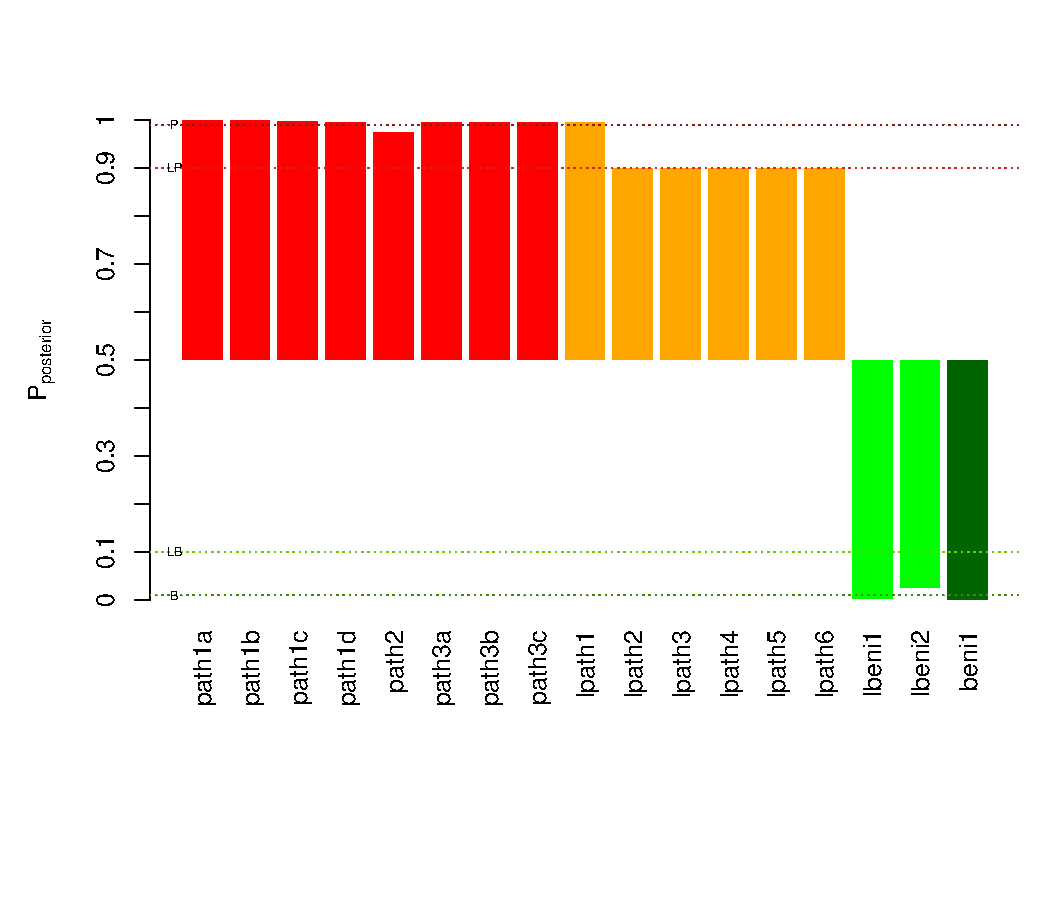
\includegraphics{tavtigian-002}

The same observations that Tavtigian et al. make stick out here as well:
Rule `path2' as defined in the ACMG guidelines is not strong enough; rule `lpath1' is
too strong; and rule `lbeni1' is too strong.

\subsection*{A deeper exploration of parameter choice}

Now, let's explore the effects of the different modeling parameters ourselves.

Indeed, choosing any other X than 2 results in violation of criterion (A), by
skewing the values of equivalent rules further from each other.

\begin{Schunk}
\begin{Sinput}
> layout(cbind(1,2))
> thresholds <- calcThresholds(LLRpvst,X=1.8)
> comboPosts <- llr2post(calcComboLLRs(thresholds),prior)
> plotRules(comboPosts,main="X=1.8")
> thresholds <- calcThresholds(LLRpvst,X=2.2)
> comboPosts <- llr2post(calcComboLLRs(thresholds),prior)
> plotRules(comboPosts,main="X=2.2")
\end{Sinput}
\end{Schunk}
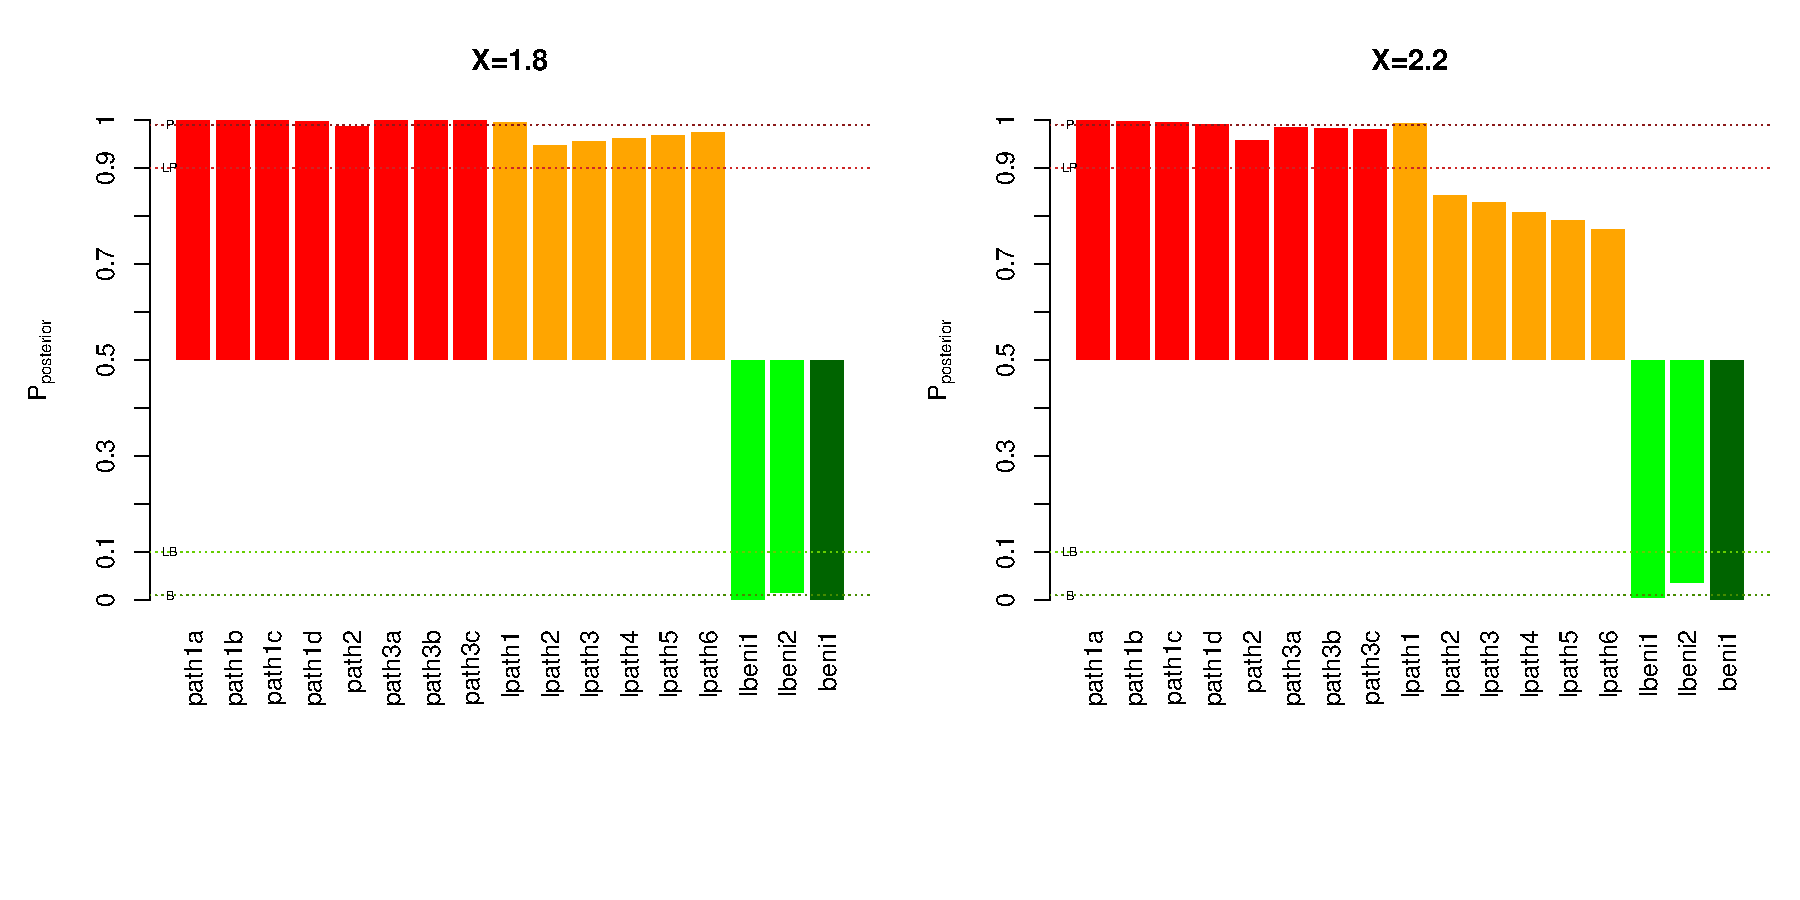
\includegraphics{tavtigian-003}

The more we stray from $X=2$ in either direction, the more the `Likely pathogenic'
combination rules fall out of sync with each other. So we must conclude that $X$
isn't really much of a free parameter at all. Only $X=2$ is a choice that can
fulfill our criteria.

As for $OP_{PVSt}$ and $P_{prior}$, we can see that both primarily affect
overall scale of the rule posteriors. Thus, only certain
combinations of the two can be expected to fulfill criteria (B) and (C). We can
actually derive a precise relationship between the two that allows us to strike
this balance by making using the likely pathogenic combination rules as a guide.
Since they must achieve a posterior of $P_{post}=90\%$, the following must hold:

$$
\frac{LLR_{PVst}}{2}+\frac{LLR_{PVst}}{4} + \log(\frac{P_{prior}}{1-P_{prior}})
 = \log(\frac{P_{post}}{1-P_{post}})
$$

If we solve for $LLR_{PVst}$:

$$
LLR_{PVst} = \frac{4}{3} \log\left( \frac{P_{post}(1-P_{prior})}{P_{prior}(1-P_{post})} \right)
$$

Let's test this:

\begin{Schunk}
\begin{Sinput}
> #function to calculate the optimal LLRpvst from the prior
> optiLLR <- function(prior,posterior=0.9) {
+ 	log10(posterior*(1-prior)/(prior*(1-posterior)))*4/3
+ }
> layout(cbind(1,2))
> prior <- 0.01
> LLRpvst <- optiLLR(prior)
> thresholds <- calcThresholds(LLRpvst,X)
> comboPosts <- llr2post(calcComboLLRs(thresholds),prior)
> plotRules(comboPosts,main="prior=0.01")
> prior <- 0.3
> LLRpvst <- optiLLR(prior)
> thresholds <- calcThresholds(LLRpvst,X)
> comboPosts <- llr2post(calcComboLLRs(thresholds),prior)
> plotRules(comboPosts,main="prior=0.3")
\end{Sinput}
\end{Schunk}
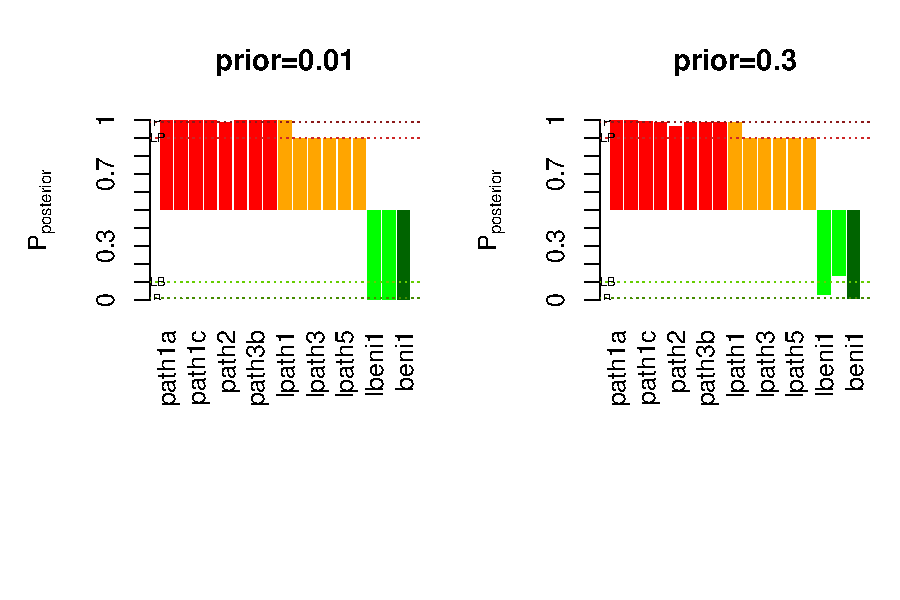
\includegraphics{tavtigian-004}

Indeed it looks like all rules except for the problematic ones already identified
by Tavtigian et al themselves remain consistent.

Having derived this relationship also lets us figure out why Tavtigian et al.
settled on $OP_{PVSt}=350$. It is numerically very close to the optimal solution
for a prior of 0.1:

\begin{Schunk}
\begin{Sinput}
> 10^optiLLR(0.1)
\end{Sinput}
\begin{Soutput}
[1] 350.4666
\end{Soutput}
\end{Schunk}

Now, lets see what the relationship between the prior and the LLR evidence
thresholds looks like in graphical form. I am highlighting Tavtigian's parameter choice in the plot as well.


\begin{Schunk}
\begin{Sinput}
> priors <- seq(0.005,0.5,0.005)
> LLRpvst <- optiLLR(priors)
> plot(priors,LLRpvst,type="l",
+ 	xlab="prior",ylab="LLR threshold",
+ 	ylim=c(-3,5)
+ )
> lines(priors,LLRpvst/2,col=2)
> lines(priors,LLRpvst/4,col=3)
> lines(priors,LLRpvst/8,col=4)
> lines(priors,-LLRpvst/8,col=4)
> lines(priors,-LLRpvst/2,col=2)
> abline(h=0,lty="dashed")
> grid()
> legend("topright",
+ 	c("Very Strong","Strong",
+ 		"Moderate","Supporting"),
+ 	col=c(1:4),lty=1
+ )
> #Highlight Tavtigian's parameter set
> points(0.1,log10(350))
> text(0.1,log10(350),"Tavtigian",pos=3)
> 
\end{Sinput}
\end{Schunk}
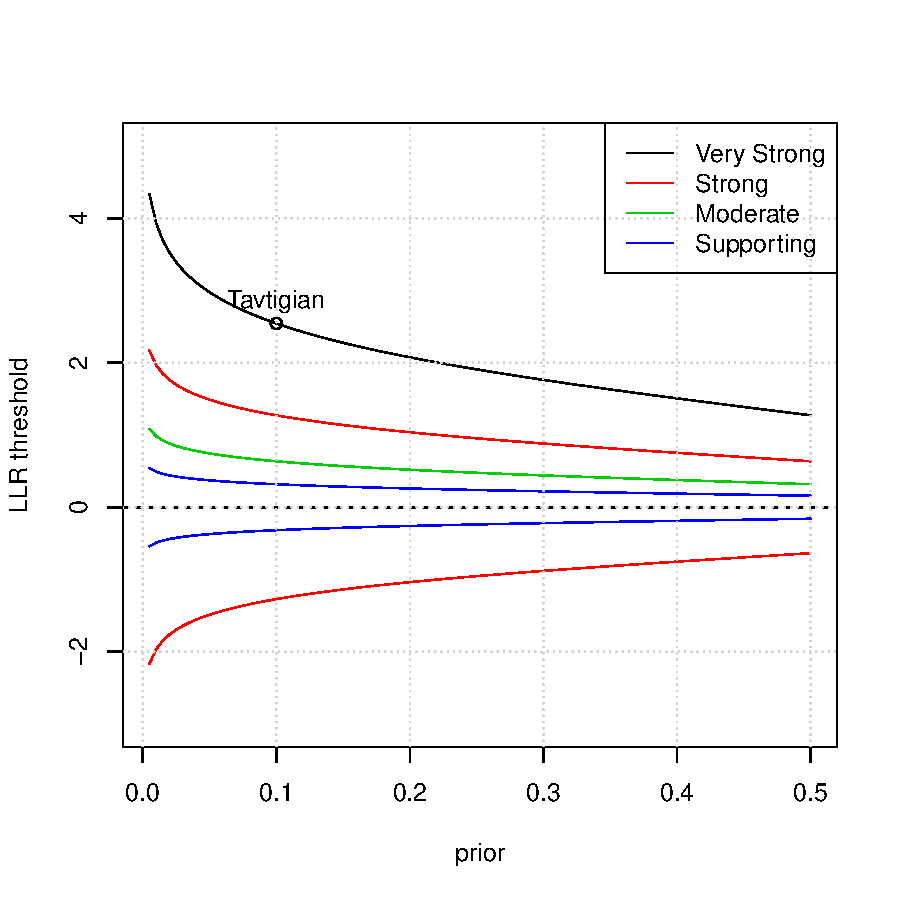
\includegraphics{tavtigian-006}

Finally let's look at this in the form of a table

\begin{Schunk}
\begin{Sinput}
> priors <- seq(0.05,0.5,0.05)
> LLRpvst <- optiLLR(priors)
> llrThresholds <- data.frame(prior=priors,patho.Vstr=LLRpvst,patho.str=LLRpvst/2,
+   patho.mod=LLRpvst/4,patho.sup=LLRpvst/8
+ )
> llrThresholds
\end{Sinput}
\begin{Soutput}
   prior patho.Vstr patho.str patho.mod patho.sup
1   0.05   2.977328 1.4886641 0.7443320 0.3721660
2   0.10   2.544647 1.2723233 0.6361617 0.3180808
3   0.15   2.276760 1.1383801 0.5691901 0.2845950
4   0.20   2.075070 1.0375350 0.5187675 0.2593838
5   0.25   1.908485 0.9542425 0.4771213 0.2385606
6   0.30   1.762959 0.8814795 0.4407398 0.2203699
7   0.35   1.630784 0.8153919 0.4076959 0.2038480
8   0.40   1.507112 0.7535558 0.3767779 0.1883890
9   0.45   1.388524 0.6942618 0.3471309 0.1735654
10  0.50   1.272323 0.6361617 0.3180808 0.1590404
\end{Soutput}
\end{Schunk}

\subsection*{Conclusions}

Of the three modeling parameters Tavtigian et al use, only one is really a
free parameter: The prior probability of pathogenicity. From it the the optimal
LLR thresholds of all the evidence levels can be derived such as to yield the
best compatibility with the ACMG ruleset.

This raises the question whether prior should probably be chosen separately
for each gene, based on the best guess of the incidence rate of pathogenic
variants in the gene.

\end{document}
